\documentclass[12pt]{report}

% ==============================================================================
% PACKAGES
% ==============================================================================

\usepackage[a4paper,margin=1in]{geometry}
\usepackage[T1]{fontenc}
\usepackage[utf8]{inputenc}
\usepackage{lmodern}
\usepackage{microtype}

\usepackage{amsmath,amsfonts,amssymb}
\usepackage{graphicx}
\usepackage{booktabs}
\usepackage{tabularx}
\usepackage{array}
\usepackage{listings}
\usepackage{xcolor}
\usepackage{float}
\usepackage{setspace}
\usepackage{titlesec}
\usepackage[round,authoryear]{natbib}
\usepackage{algorithm}
\usepackage{algpseudocode}
\usepackage{tikz}
\usetikzlibrary{positioning,arrows.meta,shapes.misc,fit}
\usepackage[hidelinks]{hyperref}
\usepackage[capitalise,noabbrev]{cleveref}
\usepackage[all]{nowidow}

\setstretch{1.15}
\setlength{\parskip}{0.5em}
\setlength{\emergencystretch}{3em}

% ==============================================================================
% HEADINGS
% ==============================================================================

\titleformat{\chapter}[display]
  {\normalfont\huge}
  {\chaptertitlename\ \thechapter}
  {20pt}
  {\Huge}
\titlespacing*{\chapter}{0pt}{0pt}{30pt}

\titleformat{\section}{\normalfont\Large}{\thesection}{1em}{}
\titleformat{\subsection}{\normalfont\large}{\thesubsection}{1em}{}

% ==============================================================================
% CODE STYLING
% ==============================================================================

\lstset{
  language=Python,
  basicstyle=\ttfamily\small,
  keywordstyle=\color{blue!60!black},
  commentstyle=\color{gray},
  stringstyle=\color{teal!70!black},
  breaklines=true,
  frame=single,
  backgroundcolor=\color{gray!8},
  columns=fullflexible,
  keepspaces=true,
  showstringspaces=false
}

\newcommand{\code}[1]{\texttt{#1}}

% ==============================================================================
% DOCUMENT
% ==============================================================================

\begin{document}

% ==============================================================================
% TITLE PAGE
% ==============================================================================

\begin{titlepage}
\centering
\vspace*{2cm}

{\Huge Congestion-Aware Adaptive Traffic Routing Using Dynamic Graph Optimisation and Neural Network Prediction\par}

\vspace{2cm}
{\Large Harvey Humphrey\par}

\vspace{1cm}
{\large Independent research project\par}

\vspace{0.5cm}
{\large Completed during studies toward the degree of\par}
\vspace{0.3cm}
{\Large BSc Computer Science with Artificial Intelligence\par}
\vspace{0.3cm}
{\large Oxford Brookes University\par}

\vspace{1.5cm}
{\large 2026 \quad (revised November 2026)\par}

\vfill
{\normalsize Source code:\\
\url{https://github.com/vey-git/Neural-Traffic-Routing-and-Congestion-Optimisation-System}\par}
\end{titlepage}

% ==============================================================================
% ABSTRACT
% ==============================================================================

\begin{abstract}

Congestion builds up where many vehicles' shortest routes share the same roads. This project builds a simulation of congestion-aware routing on the real road network of Oxford, extracted from OpenStreetMap with the OSMnx library and modelled as a weighted directed graph whose edge weights are travel times. Vehicles with random origins and destinations are routed with Dijkstra's algorithm or A*. The number of vehicles using each road is then counted, the travel time of every used road is increased in proportion to its usage, and every vehicle is re-routed once. Separately, a feed-forward neural network, implemented from first principles in NumPy, was trained to predict each road's congestion multiplier from five road and traffic features.

Experiments with 10 to 1,000 vehicles, and one logged run with 5,000, gave three main results. First, A* gave no advantage over Dijkstra. Its straight-line heuristic was measured in degrees of latitude and longitude while edge costs were in seconds, so the heuristic gave almost no guidance, and A* took up to about 30\% longer end to end. Second, congestion concentrated on a few corridors. In every logged run with 250 vehicles or more, the single busiest road segment carried 11--13\% of all vehicles. Re-routing changed the route of 82--91\% of vehicles in every logged run with 100 or more, and the heat-maps show congestion moving to other corridors rather than disappearing. Third, the neural network did not learn the mapping. It predicted an almost constant multiplier of about 1.02 for every road, giving a test $R^2$ of $-0.09$. The report traces this to a learning rate and weight initialisation that were too small for 1,000 epochs of full-batch gradient descent.

The report explains each result, identifies the weaknesses in the experimental design that limit what the comparisons can show, and sets out the changes needed for a fair algorithm comparison and a working congestion predictor.

\vspace{1em}
\noindent\small\textit{Revision note.} This version replaces the one first published in September 2026. The results were re-checked against the source code. Figures that came from earlier versions of the code were replaced with those produced by the final code. Tables that could not be reproduced from the code or the project's experiment log were removed. The conclusions were revised to match the evidence.
\end{abstract}

\tableofcontents
\listoffigures
\listoftables

% ==============================================================================
% CHAPTER 1: INTRODUCTION
% ==============================================================================

\chapter{Introduction}

\section{Background}

Traffic congestion is a persistent problem in urban road networks, and it tends to grow with city size \citep{chang2017traffic}. It lengthens journeys and imposes economic costs through lost time, extra fuel and vehicle idling \citep{calatayud2021congestion}.

Navigation systems usually route each vehicle along its own shortest or fastest path. When many vehicles make that choice independently, their routes overlap on the same arterial roads and junctions, which then become bottlenecks. Shortest-path algorithms such as Dijkstra's algorithm and A* are the standard tools for computing individual routes \citep{foead2021astar}, but on their own they take no account of the congestion that other vehicles' routes create. One response is congestion-aware re-routing: road costs are increased where usage is high, so that some vehicles are diverted to less-used alternatives \citep{angelelli2016proactive}.

This project builds and evaluates a simple version of that idea on the real road network of Oxford. It compares Dijkstra's algorithm with A*, studies how congestion spreads as the number of vehicles grows, and tests whether a neural network implemented from first principles can learn the congestion weighting from road features.

\section{Aim and Research Questions}

The aim is to investigate how congestion-aware edge weighting and learned congestion prediction affect the distribution of traffic on a real urban road graph. The project addresses three questions:

\begin{enumerate}
  \item[\textbf{RQ1}] Does A* reduce the computational cost of routing compared with Dijkstra's algorithm on a real city road network?
  \item[\textbf{RQ2}] How does congestion distribute across the network as the number of vehicles grows, and does one round of congestion-aware re-routing reduce it?
  \item[\textbf{RQ3}] Can a feed-forward neural network learn the congestion multiplier of a road from its features?
\end{enumerate}

\section{Objectives}

\begin{itemize}
  \item Build a weighted, directed graph of Oxford's drivable road network from OpenStreetMap data.
  \item Route simulated vehicles with Dijkstra's algorithm and with A*.
  \item Implement congestion-aware edge weighting and a re-routing step.
  \item Visualise congestion with heat-maps.
  \item Implement a feed-forward neural network, with back-propagation, from first principles.
  \item Evaluate routing behaviour and prediction quality, and identify the limits of the evaluation.
\end{itemize}

\section{Contributions}

\begin{itemize}
  \item A simulation pipeline, built with OSMnx and NetworkX, that routes vehicles across Oxford, applies congestion weighting and re-routes every vehicle once.
  \item A comparison of Dijkstra's algorithm and A* that explains why A* gave no benefit in this setting.
  \item Evidence that congestion concentrates on a small number of corridors, and that one round of simultaneous re-routing displaces bottlenecks rather than removing them.
  \item A feed-forward neural network written from scratch in NumPy, together with a diagnosis of why it failed to train.
  \item A record of the implementation problems found during development and how each was fixed.
\end{itemize}

\section{Report Structure}

\Cref{ch:background} reviews the algorithms and related work. \Cref{ch:method} sets out the model and the experimental method, and \cref{ch:implementation} describes the implementation. \Cref{ch:results} presents the results, and \cref{ch:discussion} explains them and discusses the threats to their validity. \Cref{ch:conclusion,ch:future} conclude and propose future work.

% ==============================================================================
% CHAPTER 2: BACKGROUND AND RELATED WORK
% ==============================================================================

\chapter{Background and Related Work}
\label{ch:background}

\section{Road Networks as Graphs}

A road network can be represented as a weighted directed graph in which intersections are nodes and road segments are directed edges. Each edge carries a cost, such as length or travel time. Real road networks are spatial graphs: their structure is shaped by geography, they are sparse, and much of the traffic is funnelled through a small number of highly connected arterial roads \citep{barthelemy2011spatial}. OSMnx builds such graphs directly from OpenStreetMap data \citep{boeing2017osmnx}, and NetworkX provides the graph algorithms used to analyse them \citep{hagberg2008networkx}.

\section{Dijkstra's Algorithm}

Dijkstra's algorithm finds minimum-cost paths in a graph with non-negative edge weights \citep{dijkstra1959}. It repeatedly settles the unsettled node with the lowest known distance from the source and relaxes that node's outgoing edges. Relaxation updates the distance to a neighbour $v$ of $u$ whenever
\begin{equation}
d(v) > d(u) + w(u,v),
\label{eq:relax}
\end{equation}
where $d(\cdot)$ is the shortest distance known so far and $w(u,v)$ is the weight of edge $(u,v)$. With a binary-heap priority queue, the running time is
\begin{equation}
O\big((|V| + |E|)\log |V|\big)
\end{equation}
for a graph with $|V|$ nodes and $|E|$ edges \citep{cormen2009algorithms}. Because the search expands outwards in every direction, it explores many nodes that lie away from the destination. A common refinement for single source--target queries is \emph{bidirectional} Dijkstra, which searches forwards from the source and backwards from the target at the same time and stops when the two searches meet. It typically settles far fewer nodes than a one-directional search.

\section{The A* Algorithm}

A* extends Dijkstra's algorithm with a heuristic that estimates the remaining cost to the goal \citep{hart1968astar}. Nodes are expanded in order of
\begin{equation}
f(n) = g(n) + h(n),
\label{eq:astar}
\end{equation}
where $g(n)$ is the cost of the best path found so far from the start to $n$, and $h(n)$ estimates the cost from $n$ to the goal. If $h$ is \emph{admissible}, meaning that it never overestimates the true remaining cost $h^*(n)$,
\begin{equation}
h(n) \leq h^*(n),
\end{equation}
then A* returns a minimum-cost path. If $h$ is also \emph{consistent},
\begin{equation}
h(n) \leq c(n,n') + h(n')
\end{equation}
for every edge $(n,n')$ with cost $c(n,n')$, then no node needs to be expanded more than once. The closer an admissible heuristic is to the true remaining cost, the fewer nodes A* expands. With $h \equiv 0$, A* is identical to Dijkstra's algorithm. A* is therefore never cheaper in route cost than Dijkstra's algorithm (both are optimal), and it can only be faster when the heuristic is informative \citep{hart1968astar,candra2020dijkstra}.

\section{Congestion and Route Choice}

\citet{wardrop1952} distinguished two ways in which traffic can be distributed across a network. Under the first principle, \emph{user equilibrium}, every driver uses a route that is fastest for them given everyone else's choices, so no driver can improve their journey by switching. Under the second, \emph{system optimum}, routes are chosen to minimise the total travel time of all drivers. The two generally differ: drivers acting independently do not minimise total delay. Computing a user equilibrium is an iterative process, because each round of route changes alters the congestion that the next round responds to \citep{sheffi1985urban}. Proactive route guidance systems aim to steer traffic towards better system-level outcomes by anticipating congestion before it forms \citep{angelelli2016proactive}. Planning each agent's path independently is also known to produce conflicts in multi-agent pathfinding, which is one reason that field plans paths jointly \citep{standley2010cooperative}.

Classical traffic-flow theory relates flow $q$, density $k$ and speed $v$ through
\begin{equation}
q = k v,
\end{equation}
with speed falling as density rises \citep{greenshields1935}. The simulation in this project does not model speed or density directly. It approximates congestion by counting how many vehicle routes use each road segment (\cref{sec:weighting}). Congestion is also concentrated by the network's structure: roads that connect large parts of the network attract many shortest paths, and so tend to remain congested whichever routes individual drivers choose \citep{barthelemy2011spatial,calatayud2021congestion}.

\section{Neural Networks for Congestion Prediction}

Artificial neural networks are built from simple connected units that each compute a weighted sum of their inputs and apply a non-linear activation function \citep{krogh2008ann}. In a feed-forward network, information flows from an input layer through one or more hidden layers to an output layer. For neuron $j$ with inputs $x_i$, the weighted input and activation are
\begin{equation}
z_j = \sum_{i=1}^{n} w_{ij} x_i + b_j, \qquad a_j = f(z_j),
\end{equation}
where $w_{ij}$ are weights, $b_j$ is a bias and $f$ is the activation function. The weights are learned by gradient descent, with gradients computed by back-propagation \citep{goodfellow2016deep}. Feed-forward networks can approximate non-linear regression functions \citep{arulampalam2003generalized} and were applied to traffic control and congestion prediction as early as the 1990s \citep{gilmore1995neural}.

Short-term traffic forecasting has since moved towards models that capture time and network structure \citep{vlahogianni2004short,vlahogianni2014short}. Recurrent networks model sequences of traffic states. Graph neural networks pass information along the edges of the road graph, which suits traffic data defined on a network \citep{wu2021comprehensive,jiang2022gnn}. These models generally need more data and computation than a feed-forward network. Reinforcement learning, in which an agent learns a policy through interaction with an environment \citep{sutton2018reinforcement}, has also been proposed for adaptive routing. This project uses a feed-forward network because it can be implemented and understood fully from first principles, and because the prediction task studied here has no time dimension.

\section{Hopfield Networks}

Hopfield networks were considered as an alternative way of framing route selection as optimisation. A Hopfield network is a recurrent network of fully connected neurons whose state evolves to reduce an energy function \citep{hopfield1982},
\begin{equation}
E = -\frac{1}{2}\sum_{i,j} w_{ij} x_i x_j + \sum_{i} \theta_i x_i,
\end{equation}
where $w_{ij}$ is the weight between neurons $i$ and $j$, $x_i$ is the state of neuron $i$ and $\theta_i$ is its threshold. Routing constraints such as path continuity and congestion penalties can in principle be encoded in the weights, so that low-energy states correspond to good routes. The approach was not adopted, for three reasons. The network converges to a fixed state, so every change in congestion requires the optimisation to be run again. It is prone to settling in local minima. And a fully connected network needs $O(n^2)$ weights for $n$ neurons, which scales poorly to a city road network.

% ==============================================================================
% CHAPTER 3: METHODOLOGY
% ==============================================================================

\chapter{Methodology}
\label{ch:method}

\section{Research Approach}

The project uses simulation. A simulation allows routing behaviour to be studied under controlled traffic loads on a real road network, without access to live traffic data. A real network extracted from OpenStreetMap was used in preference to a synthetic graph, so that the results reflect the irregular structure of an actual city.

\section{Graph Model}

The road network is a directed multigraph $G = (V, E)$, where $V$ is the set of intersections and $E$ the set of directed road segments. Parallel edges are allowed, because two intersections can be joined by more than one road. Each edge $e$ has a positive cost given by the weighting function
\begin{equation}
w : E \rightarrow \mathbb{R}^{+},
\end{equation}
where $w(e)$ is the travel time of the segment in seconds. Road networks are sparse: each intersection connects to only a few others, so $|E| \ll |V|^2$.

\section{Route Choice and the System Objective}

If $f_e$ is the number of vehicles using edge $e$ and $w_e$ its congestion-adjusted travel time, the total travel time across the network is
\begin{equation}
J = \sum_{e \in E} w_e f_e .
\label{eq:J}
\end{equation}
Minimising $J$ gives the system optimum described in \cref{ch:background}. The simulation does not solve this problem. Each vehicle chooses its own fastest route given the edge weights at the time, which is the behaviour behind a user equilibrium. Re-routing is performed once rather than repeated until routes stop changing, so the simulation approximates the first step towards a user equilibrium rather than reaching one. Road capacity is not modelled: congestion is measured relative to the average usage of the network, not relative to how many vehicles a road can carry.

\section{Congestion Weighting}
\label{sec:weighting}

After all initial routes have been computed, the usage $V_e$ of each edge is the number of vehicle routes that include it. Let $\bar{V}$ be the mean usage over the edges used by at least one vehicle. The relative usage of edge $e$ is
\begin{equation}
r_e = \frac{V_e}{\max(\bar{V}, 1)} .
\label{eq:ratio}
\end{equation}
Each used edge receives a congestion multiplier
\begin{equation}
m_e = \min(1 + 0.35\, r_e,\; 5),
\label{eq:multiplier}
\end{equation}
which is damped by a factor of 0.95 when it is applied to the edge's baseline travel time $w_e^{\text{base}}$:
\begin{equation}
w_e = w_e^{\text{base}}\,\big(1 + 0.95\,(m_e - 1)\big) = w_e^{\text{base}}\,(1 + 0.3325\, r_e) \quad \text{for } r_e \le 11.4 .
\label{eq:effective}
\end{equation}
The multiplier therefore rises linearly with relative usage, from about 1.3 for an edge with average usage to a maximum of 4.8. Edges that no vehicle uses keep their baseline travel time. The multiplier is always applied to the stored baseline, never to an already-adjusted weight, so repeated updates cannot compound (\cref{sec:debugging}). Earlier versions of the project used a stepped multiplier with fixed thresholds. The final version uses the continuous form above.

\section{Neural Network Formulation}
\label{sec:nn-method}

The network predicts the congestion multiplier $m_e$ of \cref{eq:multiplier} from five features of each edge:

\begin{enumerate}
  \item edge usage $V_e$;
  \item road length in metres;
  \item speed limit in km/h;
  \item a derived ``nearby congestion'' feature, $V_e \times (\text{length}/100) \times (50/\text{speed})$. Despite its name, this combines the edge's own usage, length and speed and does not use neighbouring edges;
  \item road type, encoded as an integer from 0 (motorway) to 5 (residential).
\end{enumerate}

Training examples are exported after re-routing, one for every edge in the graph, whether or not it was used. Unused edges have $V_e = 0$ and therefore a target of exactly 1.0. The architecture has five inputs, two hidden layers of 16 and 8 neurons with ReLU activation, and a single linear output. Training minimises the mean squared error
\begin{equation}
L = \frac{1}{n}\sum_{i=1}^{n}(y_i - \hat{y}_i)^2
\end{equation}
by full-batch gradient descent. The gradient for the output weights follows from the chain rule,
\begin{equation}
\frac{\partial L}{\partial W_3} = \frac{\partial L}{\partial \hat{y}}\,\frac{\partial \hat{y}}{\partial Z_3}\,\frac{\partial Z_3}{\partial W_3},
\end{equation}
and the error term for hidden layer $l$ is propagated backwards as
\begin{equation}
\delta^{(l)} = \big(W^{(l+1)}\big)^{\!\top} \delta^{(l+1)} \odot f'\big(z^{(l)}\big),
\end{equation}
where $\odot$ is element-wise multiplication and $f'$ is the derivative of ReLU, equal to 1 for positive inputs and 0 otherwise. Every weight matrix is updated with
\begin{equation}
W := W - \eta \frac{\partial L}{\partial W},
\end{equation}
where $\eta$ is the learning rate.

Before training, the examples are shuffled and split into 80\% for training and 20\% for testing. Input features are standardised with the training set's mean $\mu$ and standard deviation $\sigma$, $x' = (x - \mu)/\sigma$. Targets are scaled to $[0, 1]$ with $y' = (y - y_{\min})/(y_{\max} - y_{\min})$. Predictions are converted back to the original scale before evaluation. Examples with targets outside $(0.8, 5.0)$ are removed.

\section{Experimental Setup}

The road network is Oxford's drivable network, obtained with OSMnx's \code{graph\_from\_place} for the place name ``Oxford, England'' and the network type \code{drive}. Edge speeds and travel times are added by OSMnx from OpenStreetMap speed limits, with imputed values where none are recorded. For each run, $N$ vehicles are created, each with an origin and a destination drawn uniformly at random from the graph's nodes. A new pair is drawn if no path exists. Each run uses a single routing algorithm for the initial routes and then performs the congestion update and one round of re-routing. No random seed was fixed, so every run draws a different set of vehicles. Runs were performed for vehicle counts between 10 and 1,000, with one logged run of 5,000. The software versions were Python with OSMnx 1.9.3, NetworkX 3.3, NumPy 2.1.1, Pandas 2.2.2 and Matplotlib 3.9.2.

\section{Evaluation Metrics}

\Cref{tab:metrics} defines each metric exactly as it is computed in the code. Routing metrics are recorded after re-routing.

\begin{table}[htbp]
\centering
\caption{Evaluation metrics, as computed in the code}
\label{tab:metrics}
\small
\begin{tabularx}{\textwidth}{>{\raggedright\arraybackslash}p{3.6cm}X}
\toprule
Metric & Definition \\
\midrule
Mean edge usage & Total number of edge traversals across all routes, divided by the number of distinct edges used. \\
Maximum edge usage & The largest number of vehicle routes that include any single edge. \\
Average travel cost & Mean route travel time in seconds, evaluated with the congestion-adjusted weights. \\
Re-routed vehicles & Number of vehicles whose route after re-routing differs from their initial route. \\
Runtime & Wall-clock time for the whole run in seconds: graph construction, vehicle generation and routing, congestion update, re-routing, two heat-map renders and data export. \\
Route length & Mean number of nodes on the initial routes. The code records this as \code{nodes\_explored}, but it measures the length of the route returned, not the number of nodes the search examined. \\
MSE, RMSE, MAE & Mean squared error, its square root, and mean absolute error of the network's predictions on the test set, in the original units of the multiplier. \\
$R^2$ & Coefficient of determination on the test set: $1 - \sum (y-\hat{y})^2 / \sum (y - \bar{y})^2$. A value of 0 means the model does no better than always predicting the mean target; a negative value means it does worse \citep{chicco2021coefficient}. \\
\bottomrule
\end{tabularx}
\end{table}

% ==============================================================================
% CHAPTER 4: SYSTEM DESIGN AND IMPLEMENTATION
% ==============================================================================

\chapter{System Design and Implementation}
\label{ch:implementation}

\section{Pipeline}

\Cref{fig:pipeline} shows the simulation pipeline. Each run builds the graph, generates vehicles, computes initial routes, applies the congestion weighting, re-routes every vehicle once, and then records metrics, heat-maps and training data. The neural network is trained separately on the exported data. The code can use the network's prediction in place of the formula in \cref{eq:multiplier}, but that option is switched off in the main program and is not evaluated in this report.

\begin{figure}[htbp]
\centering
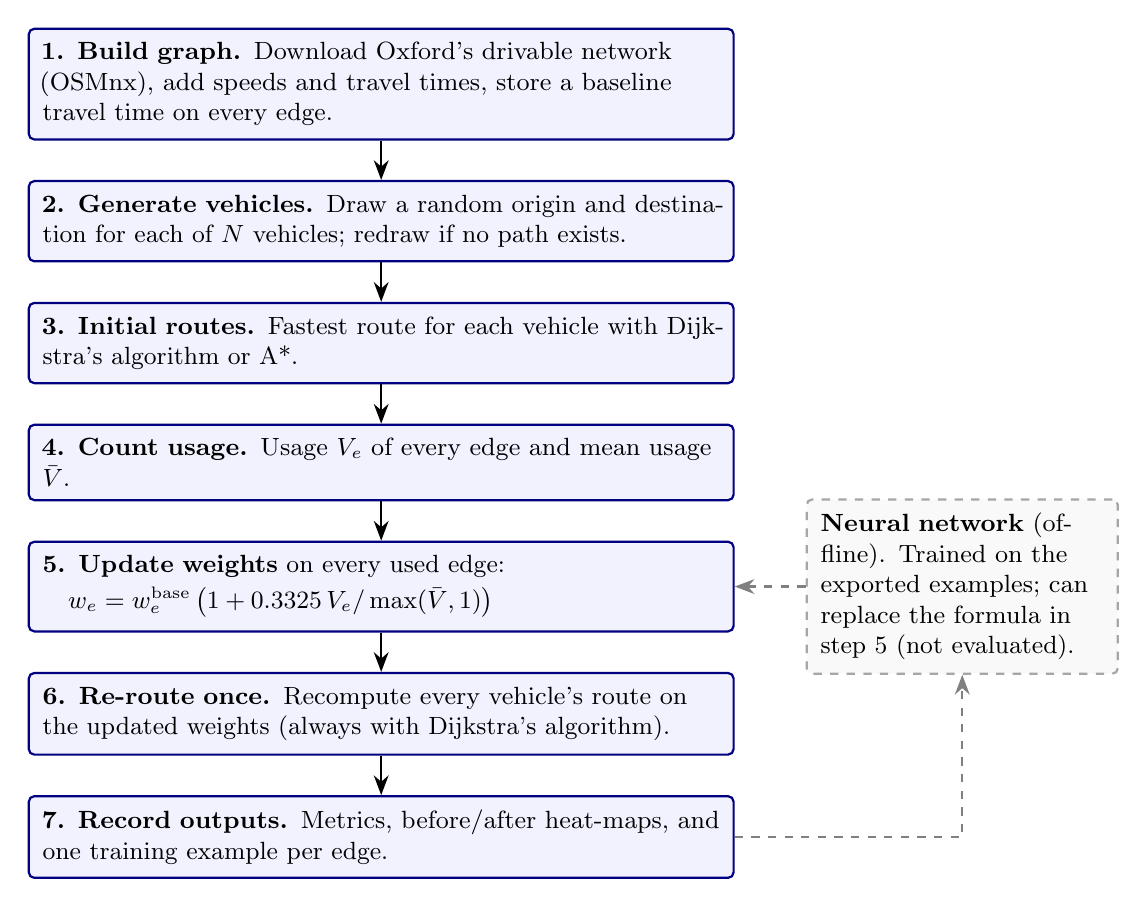
\begin{tikzpicture}[
  node distance=5mm,
  stage/.style={rectangle, rounded corners=2pt, draw=blue!50!black, fill=blue!5, thick,
               text width=8.6cm, align=left, inner sep=5pt, font=\small},
  side/.style={rectangle, rounded corners=2pt, draw=gray!70, dashed, fill=gray!5, thick,
               text width=3.6cm, align=left, inner sep=5pt, font=\small},
  arr/.style={-{Stealth[length=2.5mm]}, thick}
]
\node[stage] (s1) {\textbf{1. Build graph.} Download Oxford's drivable network (OSMnx), add speeds and travel times, store a baseline travel time on every edge.};
\node[stage, below=of s1] (s2) {\textbf{2. Generate vehicles.} Draw a random origin and destination for each of $N$ vehicles; redraw if no path exists.};
\node[stage, below=of s2] (s3) {\textbf{3. Initial routes.} Fastest route for each vehicle with Dijkstra's algorithm or A*.};
\node[stage, below=of s3] (s4) {\textbf{4. Count usage.} Usage $V_e$ of every edge and mean usage $\bar{V}$.};
\node[stage, below=of s4] (s5) {\textbf{5. Update weights} on every used edge:\\[2pt] \hspace*{1em}$w_e = w_e^{\text{base}}\,\big(1 + 0.3325\, V_e/\max(\bar{V},1)\big)$};
\node[stage, below=of s5] (s6) {\textbf{6. Re-route once.} Recompute every vehicle's route on the updated weights (always with Dijkstra's algorithm).};
\node[stage, below=of s6] (s7) {\textbf{7. Record outputs.} Metrics, before/after heat-maps, and one training example per edge.};
\node[side, right=9mm of s5] (nn) {\textbf{Neural network} (offline). Trained on the exported examples; can replace the formula in step 5 (not evaluated).};
\foreach \a/\b in {s1/s2,s2/s3,s3/s4,s4/s5,s5/s6,s6/s7} \draw[arr] (\a) -- (\b);
\draw[arr, dashed, gray] (s7.east) -| (nn.south);
\draw[arr, dashed, gray] (nn.west) -- (s5.east);
\end{tikzpicture}
\caption[Simulation pipeline]{Simulation pipeline. Solid arrows show the steps of every run; dashed arrows show the optional neural-network path, which was not evaluated.}
\label{fig:pipeline}
\end{figure}

\section{Road Network Generation}

The graph is built with OSMnx \citep{boeing2017osmnx}, which returns a NetworkX \code{MultiDiGraph}. Nodes carry longitude and latitude (\code{x}, \code{y}), and edges carry length, road type and geometry. A multigraph is needed because two intersections can be joined by several directed road segments. After adding speeds and travel times, the code copies each edge's travel time into a \code{base\_travel\_time} attribute, so congestion multipliers can always be applied to the original value:

\begin{lstlisting}
graph = ox.graph_from_place(PLACE_NAME, network_type="drive")
graph = ox.add_edge_speeds(graph)
graph = ox.add_edge_travel_times(graph)
for u, v, key, data in graph.edges(keys=True, data=True):
    data["base_travel_time"] = data["travel_time"]
\end{lstlisting}

An early version located places with free-text geographic queries. These produced approximate coordinates that sometimes fell off the road network, so the final version takes origins and destinations directly from the graph's nodes.

\section{Vehicle Generation and Routing}

Each vehicle stores its origin, its destination, the algorithm used and its route. Origins and destinations are drawn from the graph's nodes. Because parts of a real directed road network cannot reach each other, NetworkX raises \code{NetworkXNoPath} for some pairs, and the generator then draws a new pair:

\begin{lstlisting}
while not valid_route:
    start_node = random.choice(graph_nodes)
    destination_node = random.choice(graph_nodes)
    try:
        vehicle = Vehicle(graph, start_node, destination_node, algorithm)
        valid_route = True
    except nx.NetworkXNoPath:
        pass  # draw a new pair
\end{lstlisting}

Routes are computed on the \code{travel\_time} weight. For Dijkstra's algorithm the code calls \code{nx.shortest\_path}; for a single source and target, this function runs bidirectional Dijkstra. A* uses \code{nx.astar\_path} with a straight-line heuristic computed from node coordinates:

\begin{lstlisting}
route = nx.astar_path(graph, start, goal,
                      heuristic=self.heuristic, weight="travel_time")

def heuristic(self, node1, node2):
    x1, y1 = graph.nodes[node1]["x"], graph.nodes[node1]["y"]
    x2, y2 = graph.nodes[node2]["x"], graph.nodes[node2]["y"]
    return ((x1 - x2) ** 2 + (y1 - y2) ** 2) ** 0.5
\end{lstlisting}

Because \code{x} and \code{y} are longitude and latitude, this heuristic is measured in degrees, while route costs are in seconds. The consequences are analysed in \cref{sec:disc-astar}. Re-routing calls \code{nx.shortest\_path} for every vehicle, whichever algorithm produced its initial route.

\section{Congestion Weighting and Re-routing}

Edge usage is counted by walking along each route and incrementing a counter for every consecutive pair of nodes. The weights of every used edge, including all parallel edges between the same pair of nodes, are then updated as in \cref{sec:weighting}:

\begin{lstlisting}
congestion_factor = usage / max(average_edge_usage, 1)
multiplier = min(1.0 + congestion_factor * 0.35, 5.0)
updated = base_travel_time * multiplier
data["travel_time"] = base_travel_time + (updated - base_travel_time) * 0.95
\end{lstlisting}

Route generation, congestion calculation and re-routing are run as three separate stages over all vehicles. Each vehicle is re-routed once from its origin.

\section{Heat-map Visualisation}

Heat-maps colour every edge by its usage relative to the mean usage $\bar{V}$, using the categories in \cref{tab:heatmap}. Because the categories are relative, the colours show where traffic is concentrated within a single run; they do not compare absolute congestion between runs. \Cref{fig:heatmap100} shows an example with 100 vehicles. Cyan points mark vehicle positions.

\begin{table}[htbp]
\centering
\caption{Heat-map colour categories}
\label{tab:heatmap}
\begin{tabular}{ll}
\toprule
Usage relative to mean, $V_e/\bar{V}$ & Colour \\
\midrule
below 0.5 (including unused roads) & Green (low) \\
0.5 to 1.0 & Yellow (moderate) \\
1.0 to 1.5 & Orange (high) \\
1.5 and above & Red (severe) \\
\bottomrule
\end{tabular}
\end{table}

\begin{figure}[htbp]
\centering
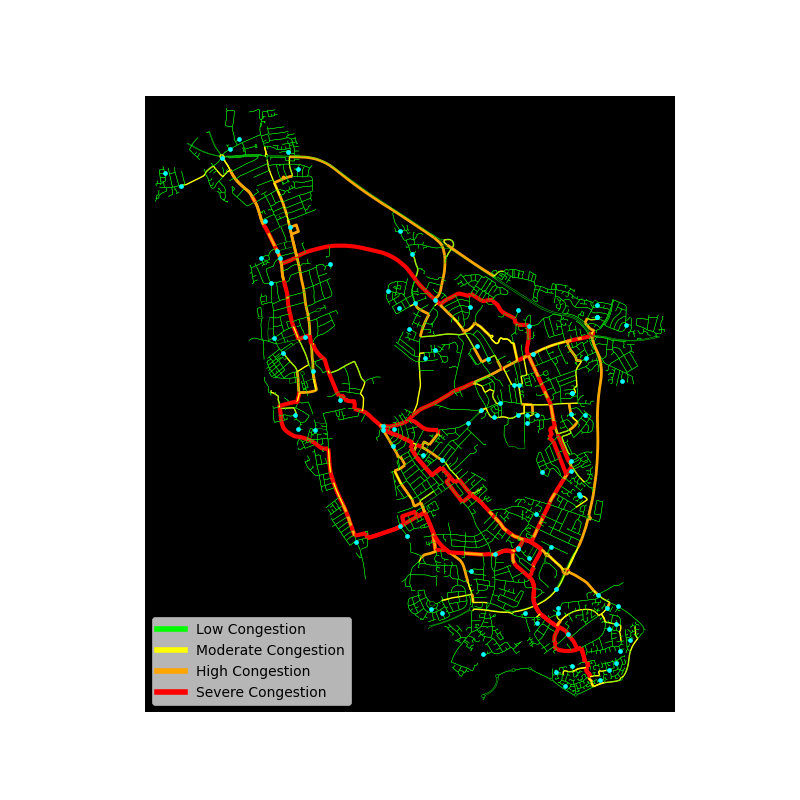
\includegraphics[width=0.62\textwidth]{figures/heatmap_100_vehicles.png}
\caption{Congestion heat-map of the Oxford road network for 100 simulated vehicles}
\label{fig:heatmap100}
\end{figure}

\section{Neural Network Implementation}

The network is implemented in NumPy without machine-learning frameworks. Forward propagation computes
\begin{equation}
\begin{aligned}
Z_1 &= X W_1 + b_1, & A_1 &= \operatorname{ReLU}(Z_1),\\
Z_2 &= A_1 W_2 + b_2, & A_2 &= \operatorname{ReLU}(Z_2),\\
\hat{y} &= A_2 W_3 + b_3 ,
\end{aligned}
\end{equation}
and back-propagation implements the gradients of \cref{sec:nn-method} directly. Weights are initialised from a standard normal distribution scaled by 0.01, and biases are initialised to zero. The trained weights and the feature- and target-scaling parameters are saved, so that the same transformations can be applied at inference time. \Cref{tab:hyper} lists the training settings.

\begin{table}[htbp]
\centering
\caption{Neural network settings}
\label{tab:hyper}
\begin{tabular}{ll}
\toprule
Setting & Value \\
\midrule
Layers & 5 -- 16 -- 8 -- 1 \\
Hidden activation & ReLU \\
Output activation & Linear \\
Weight initialisation & $0.01 \times \mathcal{N}(0,1)$; biases zero \\
Optimiser & Full-batch gradient descent \\
Learning rate $\eta$ & 0.0001 \\
Epochs & 1,000 \\
Loss & Mean squared error \\
Train/test split & 80/20 after shuffling (seed 42) \\
\bottomrule
\end{tabular}
\end{table}

\section{Implementation Problems and Fixes}
\label{sec:debugging}

Several problems were found and fixed during development.

\subsection{Disconnected graph components}
Randomly chosen origins and destinations sometimes lay in parts of the directed graph that cannot reach each other, raising \code{NetworkXNoPath}. Vehicle generation now catches the exception and draws a new pair, as shown above.

\subsection{Quadratic re-routing cost}
An early version recalculated every vehicle's route inside a loop over vehicles, so each congestion update triggered $N$ route calculations for each of $N$ vehicles: $O(N^2)$ shortest-path calls. Restructuring the simulation into three global stages (route all vehicles, update congestion, re-route all vehicles) reduced this to $2N$ calls.

\subsection{Edge indexing error}
Edges were first extracted from routes with \code{(route[1], route[i+1])} instead of \code{(route[i], route[i+1])}. Every edge was therefore paired with the route's second node, which corrupted the usage counts. The index was corrected.

\subsection{Compounding congestion weights}
Applying multipliers to already-adjusted weights made travel times grow geometrically with each update. Storing \code{base\_travel\_time} and always applying the multiplier to it fixed the problem.

\subsection{Parallel edges}
Congestion updates at first changed only the first of several parallel edges between two nodes, so vehicles could avoid the penalty by using a parallel edge. The update now loops over every edge key.

\subsection{Stale heat-maps}
Heat-maps were initially identical before and after re-routing, because usage statistics were not recomputed after re-routing. Usage is now recounted before the second heat-map is drawn.

\subsection{Input shape mismatch}
Single predictions failed with a shape error, because a feature vector was passed as a one-dimensional array. Wrapping it as a one-row matrix, \code{np.array([features])}, fixed the problem.

% ==============================================================================
% CHAPTER 5: RESULTS
% ==============================================================================

\chapter{Results}
\label{ch:results}

This chapter reports the results for each research question. Two batches of runs produced the figures: a sweep of 10, 25, 50, 75, 100, 200, 500 and 1,000 vehicles, and a sweep of 50, 100, 200 and 400 vehicles. Points in the figures are averages over repeated runs where repeats were made; the number of repeats per point was not recorded. \Cref{tab:explog} gives single runs from the project's experiment log, which make the per-run numbers concrete. Points that affect how far the comparisons can be trusted are noted as they arise and discussed in \cref{sec:validity}.

\begin{table}[htbp]
\centering
\caption[Single runs from the project's experiment log]{Single runs recorded in the project's experiment log (\code{research/experiments.md}). They were produced by an earlier version of the code, and the routing algorithm was not recorded. Two runs were made with 100 vehicles.}
\label{tab:explog}
\small
\begin{tabular}{rrrrrr}
\toprule
Vehicles & Mean edge & Max edge & Mean travel & Re-routed & Runtime \\
 & usage & usage & time (s) & vehicles & (s) \\
\midrule
5    & 1.01  & 2   & 656 & 4 (80\%)    & 1.62 \\
10   & 1.16  & 4   & 547 & 6 (60\%)    & 1.57 \\
25   & 1.58  & 6   & 616 & 22 (88\%)   & 1.64 \\
75   & 2.50  & 12  & 587 & 57 (76\%)   & 1.83 \\
100  & 2.74  & 15  & 662 & 87 (87\%)   & 1.99 \\
100  & 2.91  & 15  & 699 & 90 (90\%)   & 1.99 \\
250  & 4.36  & 33  & 643 & 206 (82\%)  & 2.58 \\
500  & 7.52  & 66  & 797 & 448 (90\%)  & 3.93 \\
750  & 9.62  & 80  & 826 & 661 (88\%)  & 4.94 \\
1000 & 11.22 & 118 & 833 & 884 (88\%)  & 6.12 \\
5000 & 38.39 & 589 & 886 & 4537 (91\%) & 24.56 \\
\bottomrule
\end{tabular}
\end{table}

\section{RQ1: Dijkstra's Algorithm and A*}

\subsection{Runtime}

\Cref{fig:runtime} shows end-to-end runtime against the number of vehicles. Runtime grows roughly linearly from about 1.8\,s at 10 vehicles. At small loads the two algorithms are indistinguishable, but A* is slower from about 50 vehicles upwards: at 1,000 vehicles it took about 10.2\,s against 7.9\,s for Dijkstra's algorithm, roughly 30\% longer. The intercept of about 1.7\,s is fixed overhead, mainly building the graph, drawing the heat-maps and exporting data, which every run pays whatever the number of vehicles.

\begin{figure}[htbp]
\centering
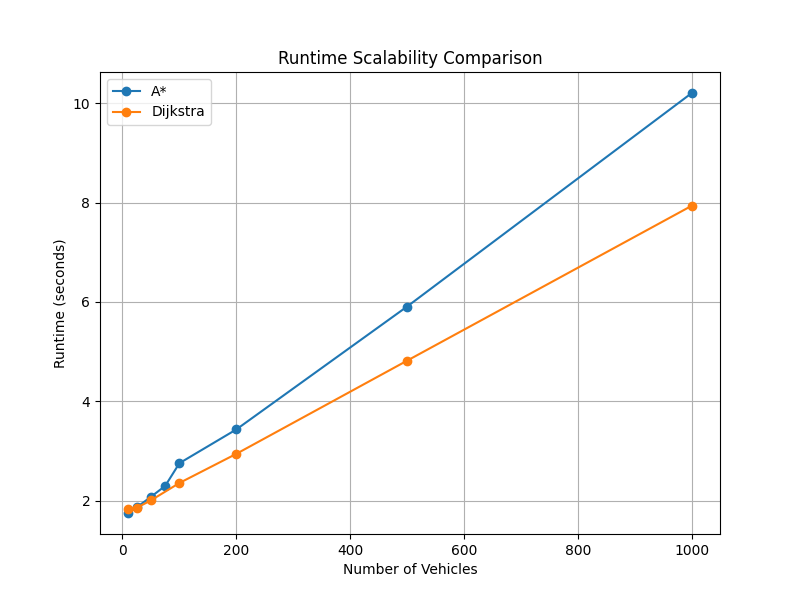
\includegraphics[width=0.72\textwidth]{figures/runtime_scalability.png}
\caption{End-to-end runtime against the number of vehicles}
\label{fig:runtime}
\end{figure}

\subsection{Route length}

\Cref{fig:routelength} shows the mean number of nodes on the initial routes. Both algorithms produce routes of about 44 to 48 nodes, with no consistent ordering between them; the two curves converge to about 46 nodes at 500 and 1,000 vehicles, where the averages are taken over more vehicles. Route length is expected to be the same for both algorithms, because both return minimum-cost routes. This metric does not measure search effort: the number of nodes each search examined was not recorded, so the data cannot show whether A* explored less of the graph.

\begin{figure}[htbp]
\centering
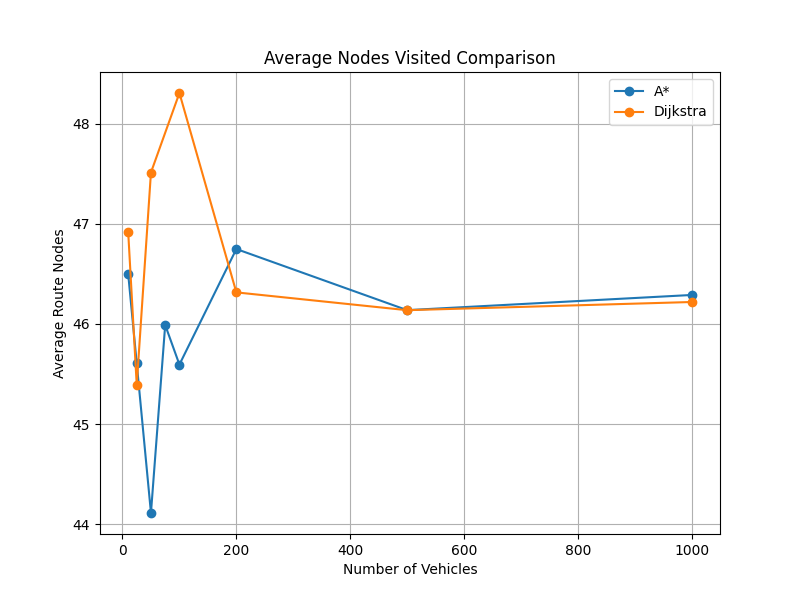
\includegraphics[width=0.72\textwidth]{figures/route_length_nodes.png}
\caption{Mean number of nodes on the initial route}
\label{fig:routelength}
\end{figure}

\subsection{Travel cost}

\Cref{fig:travelcost} shows the average travel cost after re-routing. The two curves are almost identical up to 200 vehicles and differ by about 20\,s (about 2\%) at 400 vehicles. Average travel time rises with the number of vehicles, from about 770\,s at 50 vehicles to about 900\,s at 400, as congestion weighting raises the cost of busy roads.

This comparison cannot separate the algorithms, for two reasons. First, because re-routing always uses Dijkstra's algorithm, the routes being measured were all produced by Dijkstra's algorithm, whichever algorithm computed the initial routes. Second, each run drew a different random set of vehicles. The difference seen at 400 vehicles is smaller than the 5.6\% difference between the two logged runs with 100 vehicles in \cref{tab:explog}, which used identical settings.

\begin{figure}[htbp]
\centering
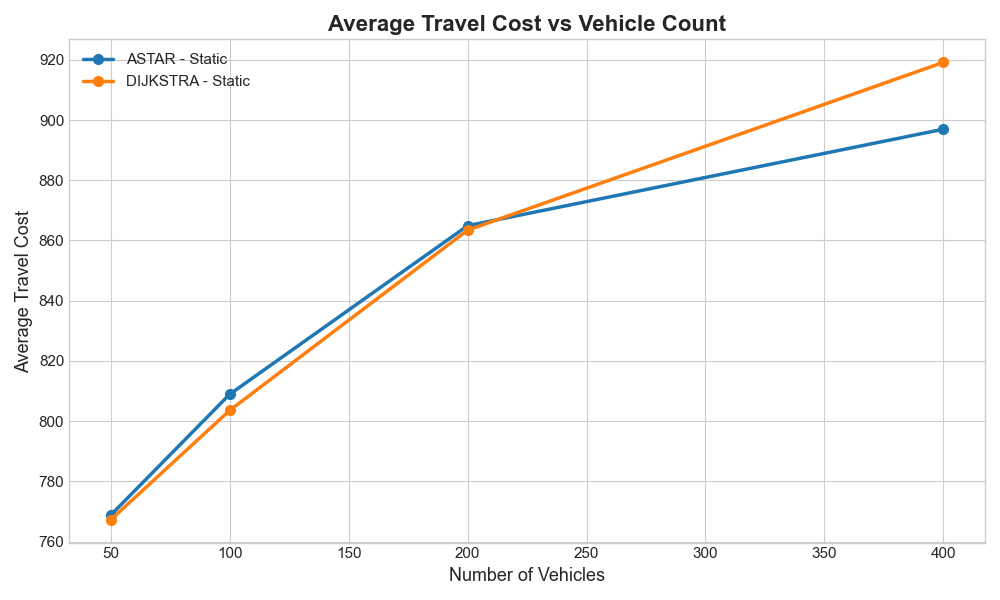
\includegraphics[width=0.78\textwidth]{figures/average_travel_cost.png}
\caption{Average travel cost (seconds) after re-routing}
\label{fig:travelcost}
\end{figure}

\section{RQ2: Congestion and Re-routing}

\subsection{Edge usage and bottlenecks}

Mean edge usage rises steadily with load, from about 2 vehicles per used edge at 50 vehicles to about 6 at 400 (\cref{fig:avgusage}), with the two algorithms' curves overlapping. Maximum edge usage grows almost linearly with the number of vehicles (\cref{fig:maxusage}), reaching about 115 to 118 at 1,000 vehicles. The experiment log shows the same pattern over a wider range: from 250 vehicles upwards, the busiest single road segment carried between 11\% and 13\% of all vehicles, including 589 of 5,000 (12\%) in the largest run. The share is stable even though re-routing has already been applied. This indicates that a small number of road segments are effectively unavoidable for a large fraction of random journeys across Oxford.

\begin{figure}[htbp]
\centering
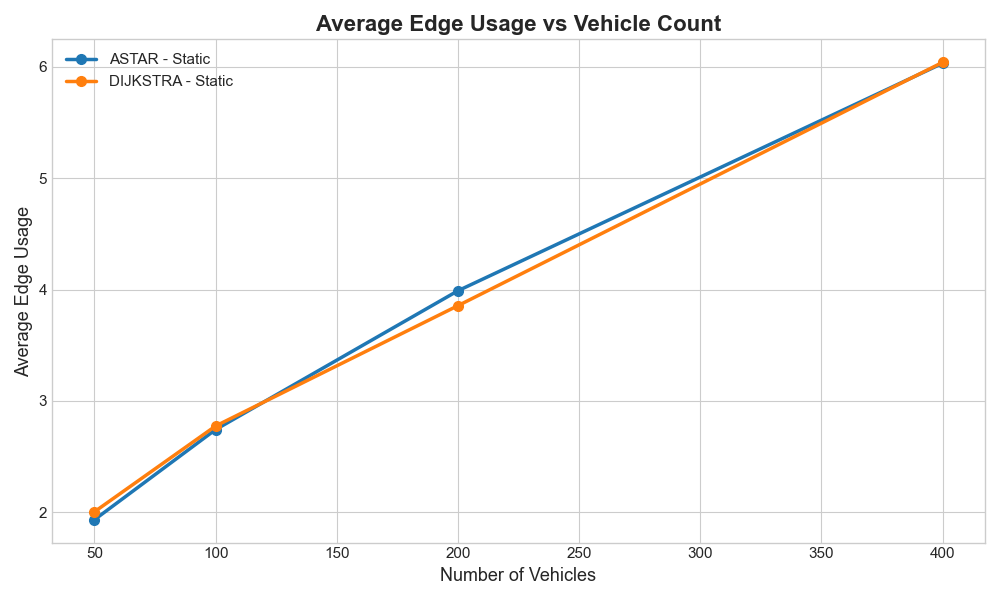
\includegraphics[width=0.78\textwidth]{figures/average_edge_usage.png}
\caption{Mean edge usage (vehicles per used edge) after re-routing}
\label{fig:avgusage}
\end{figure}

\begin{figure}[htbp]
\centering
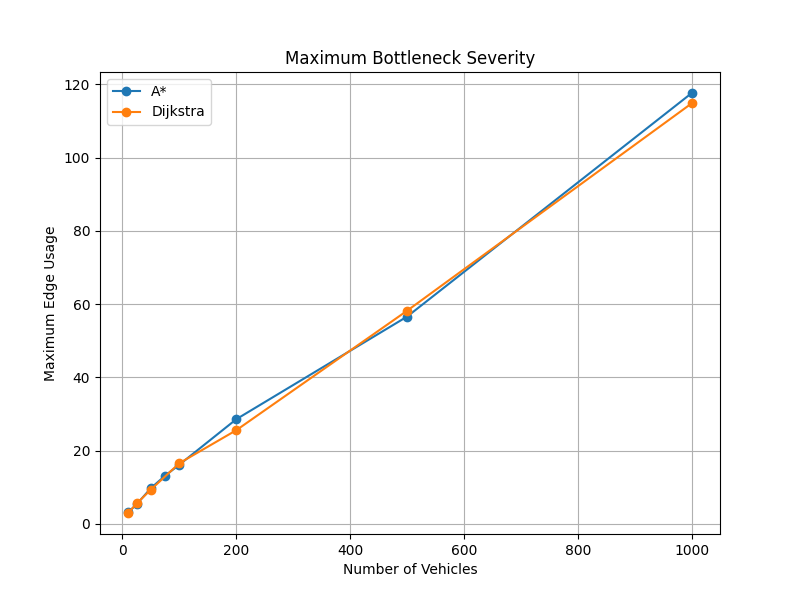
\includegraphics[width=0.72\textwidth]{figures/maximum_edge_usage.png}
\caption{Maximum edge usage after re-routing}
\label{fig:maxusage}
\end{figure}

\subsection{Re-routing}

\Cref{fig:rerouted} shows how many vehicles changed route. The number grows in proportion to the number of vehicles: roughly 80--90\% of vehicles changed route at every load in the sweep, and the logged runs show between 82\% and 91\% for every run with 100 vehicles or more (\cref{tab:explog}). Re-routing therefore did not affect only the vehicles on congested roads. It changed almost every route, at light loads as well as heavy ones. \Cref{sec:disc-reroute} explains why.

\begin{figure}[htbp]
\centering
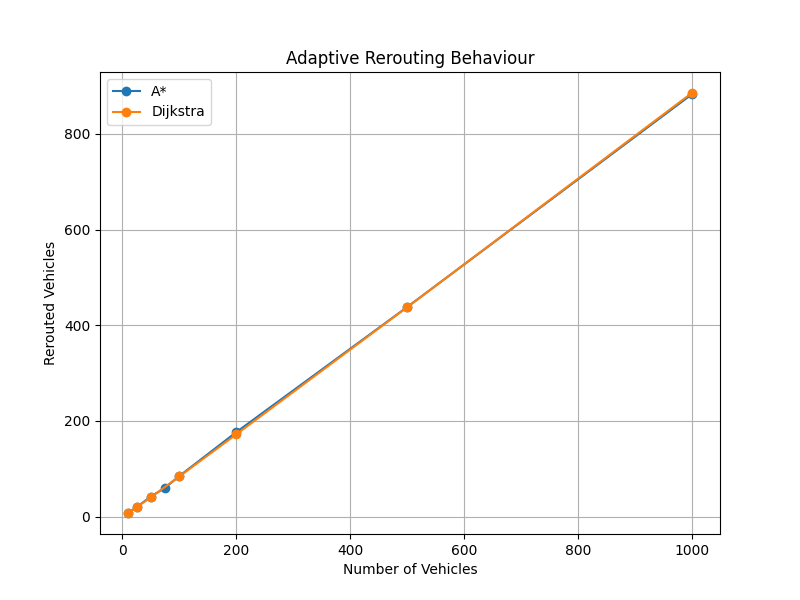
\includegraphics[width=0.72\textwidth]{figures/rerouted_vehicles.png}
\caption{Number of vehicles whose route changed after re-routing}
\label{fig:rerouted}
\end{figure}

\subsection{Distribution of congestion}

\Cref{fig:heatmaps} compares the heat-maps before and after re-routing in one run. Before re-routing, the most heavily used roads (red) are concentrated on the outer ring roads. After re-routing, much of that traffic has moved onto central and western corridors, which now carry the heaviest relative usage. Congestion was redistributed rather than removed, and the busiest roads after re-routing are still major connecting routes. Because colours are relative to each map's own mean usage, the comparison shows where traffic is concentrated in each state, not whether total congestion went up or down.

\begin{figure}[htbp]
\centering
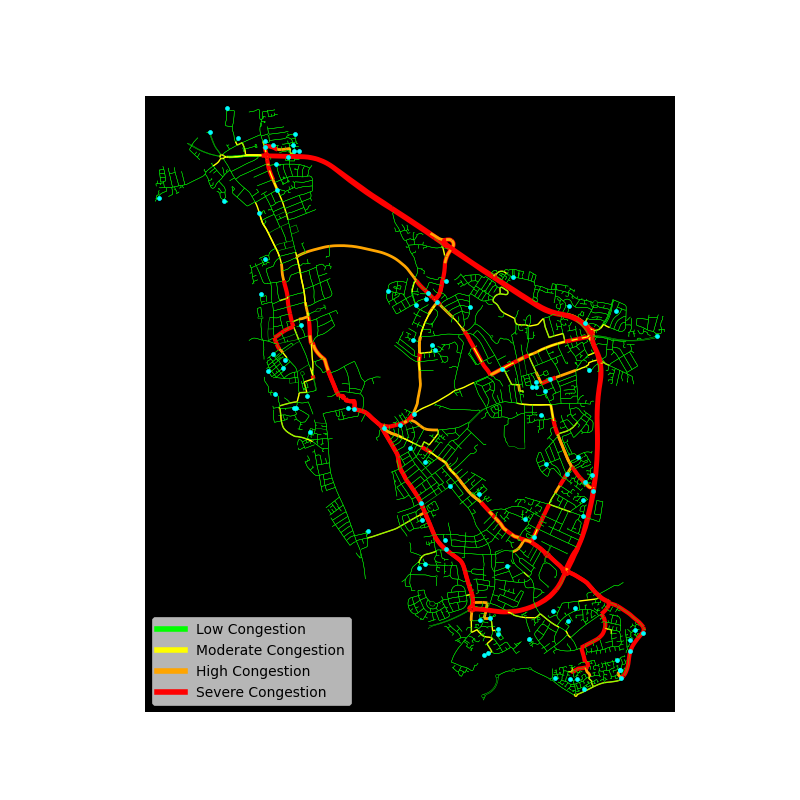
\includegraphics[width=0.48\textwidth]{figures/heatmap_before.png}\hfill
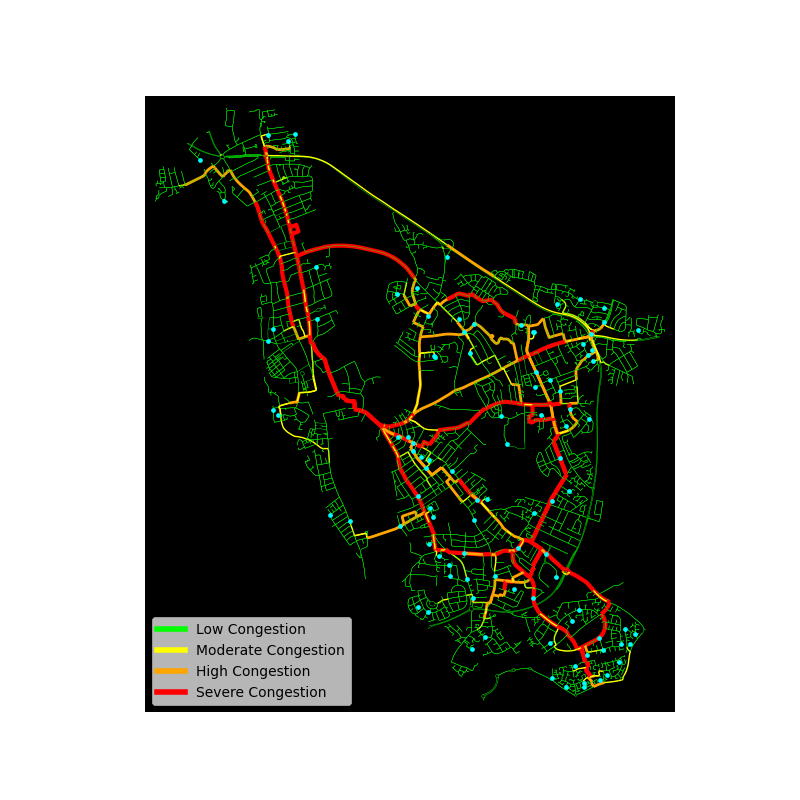
\includegraphics[width=0.48\textwidth]{figures/heatmap_after.png}
\caption{Congestion heat-maps from one run before (left) and after (right) re-routing}
\label{fig:heatmaps}
\end{figure}

\section{RQ3: Neural Network Prediction}

\Cref{fig:trainingloss} shows the training loss, measured on the normalised targets. Over 1,000 epochs it fell only from 0.00584 to 0.00561, about 4\%, and was still falling in a straight line at the end. Training had not converged.

\begin{figure}[htbp]
\centering
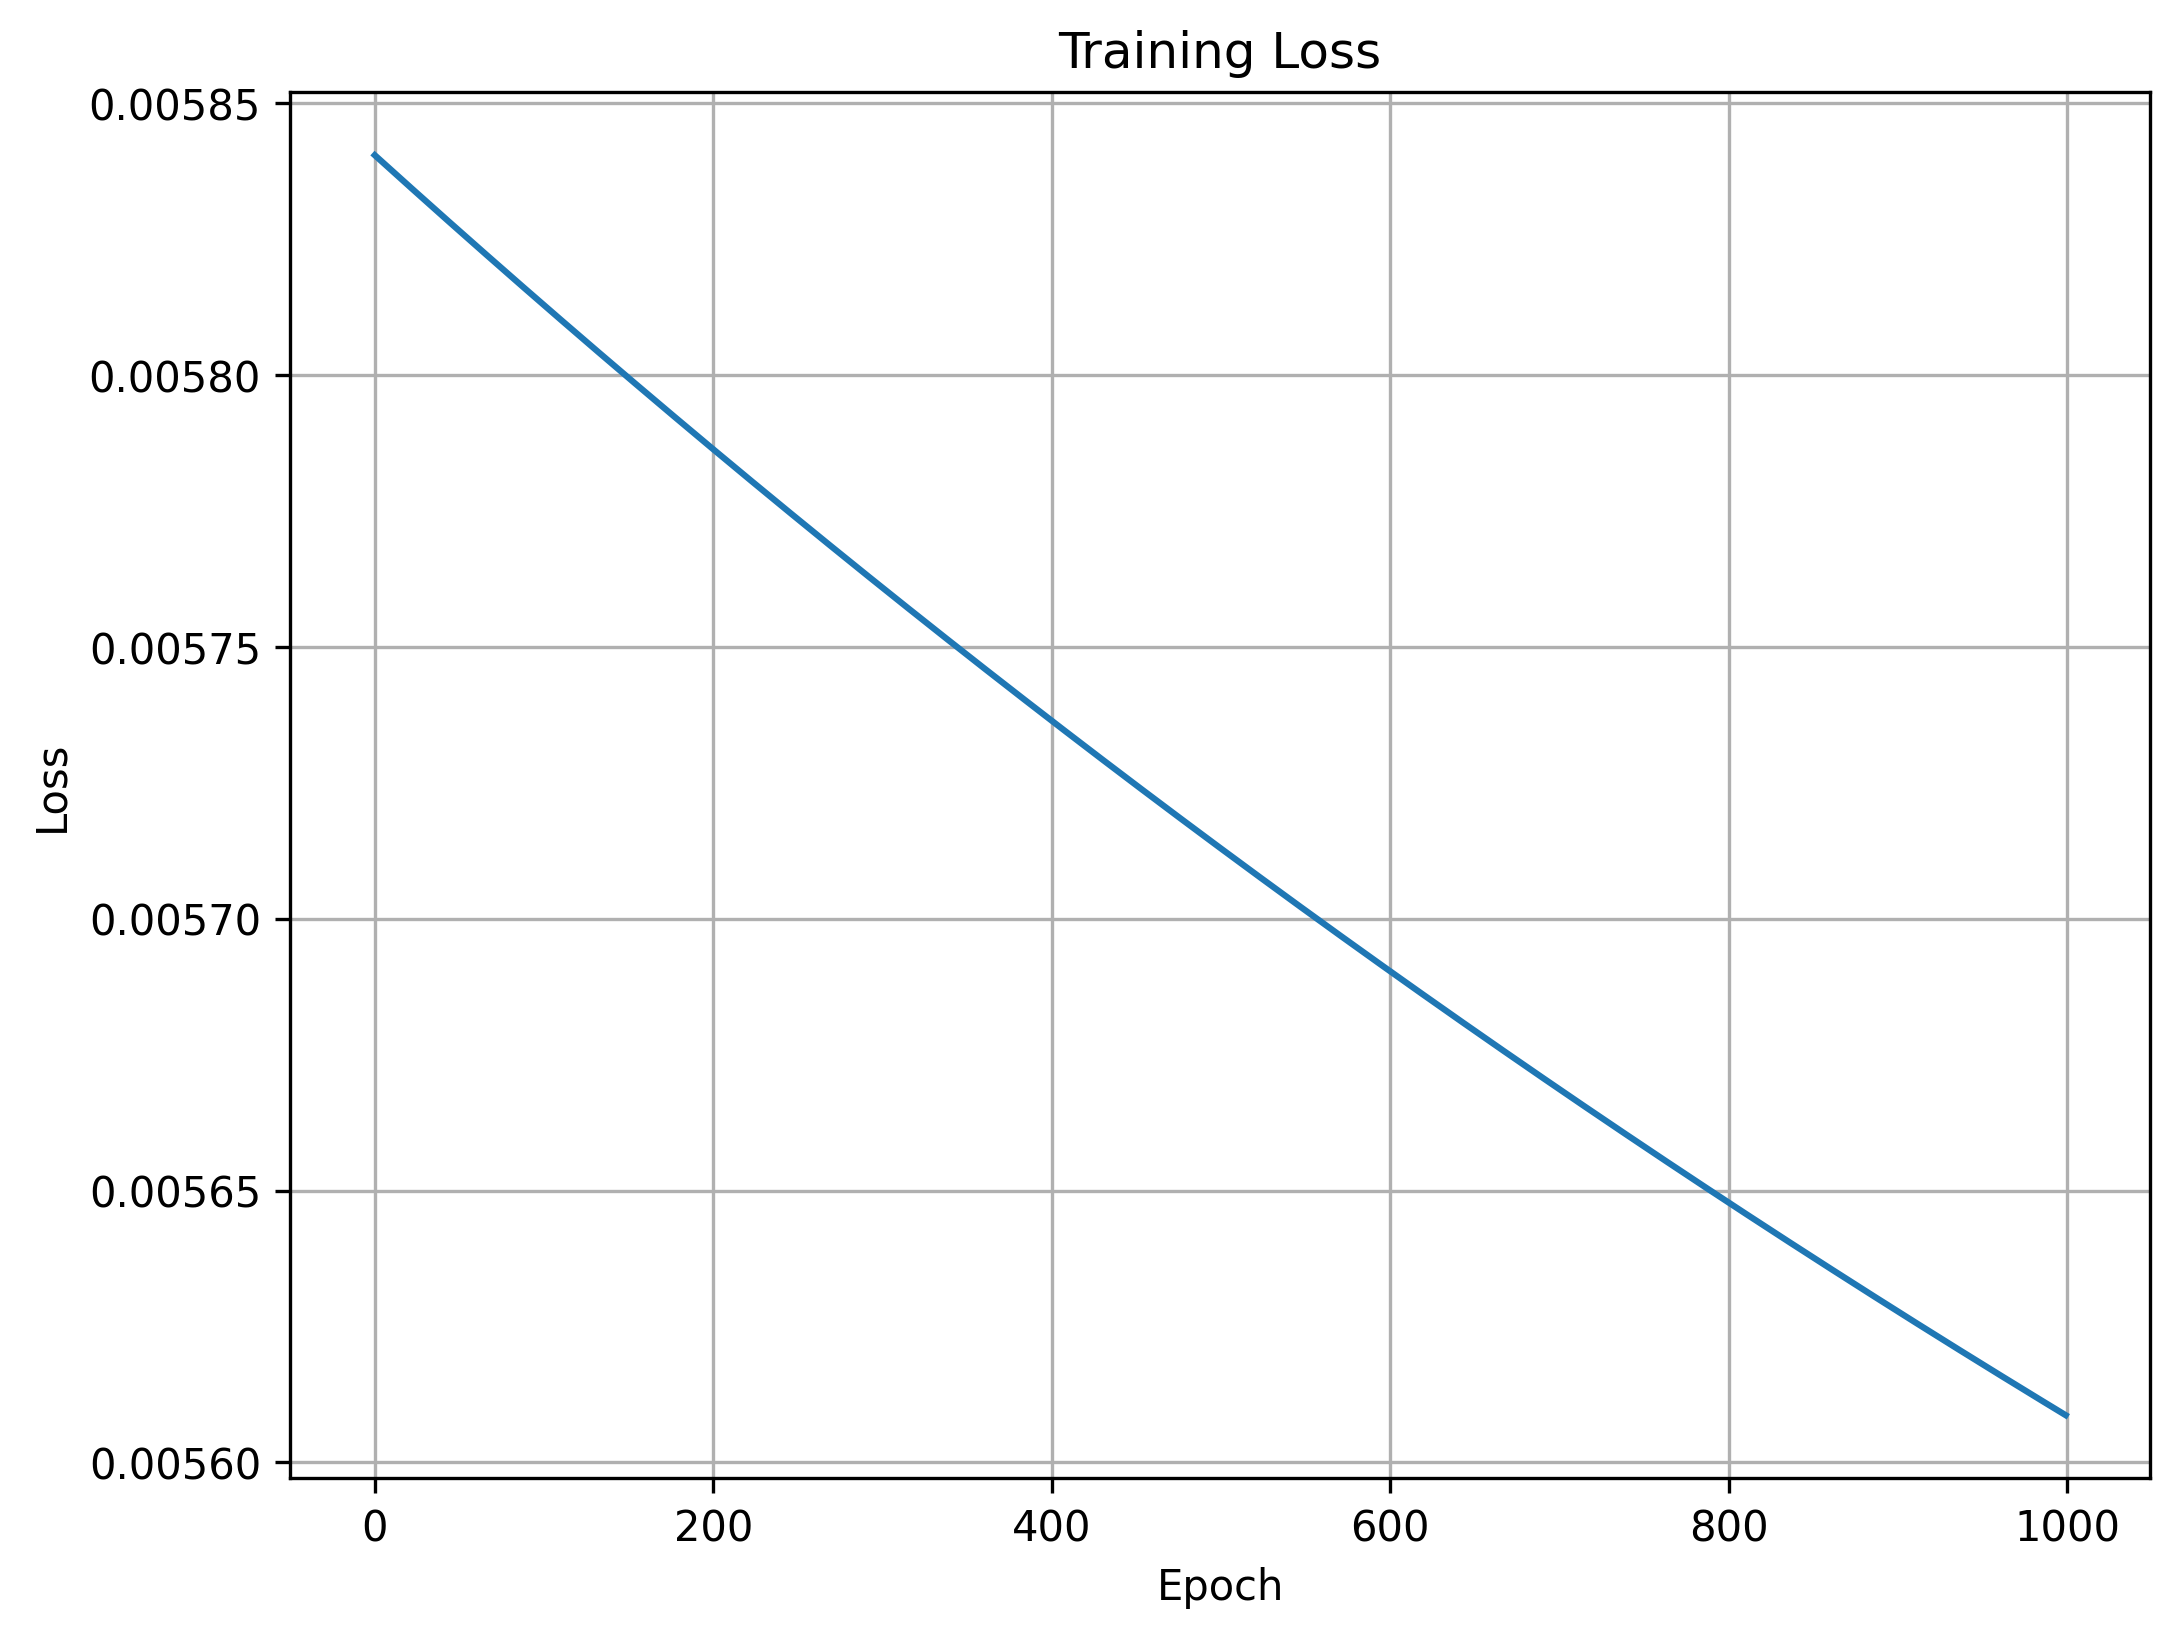
\includegraphics[width=0.66\textwidth]{figures/training_loss.png}
\caption{Training loss (mean squared error on normalised targets) over 1,000 epochs}
\label{fig:trainingloss}
\end{figure}

\Cref{fig:actualpred} plots predictions against true values on the test set. The true multipliers range from 1.0 to about 4.9, but the network predicts about 1.02 for every edge: its predictions form a flat line. \Cref{tab:nnmetrics} gives the test metrics. The mean absolute error is small (0.11) only because most targets are exactly 1.0 (unused edges), which a constant prediction of 1.02 is close to. The negative $R^2$ shows that the network does worse than simply predicting the mean target value. Treating the prediction as constant at 1.02, the MSE and $R^2$ together imply that the test targets have a mean of about 1.11, so the prediction sits below the mean.

\begin{figure}[htbp]
\centering
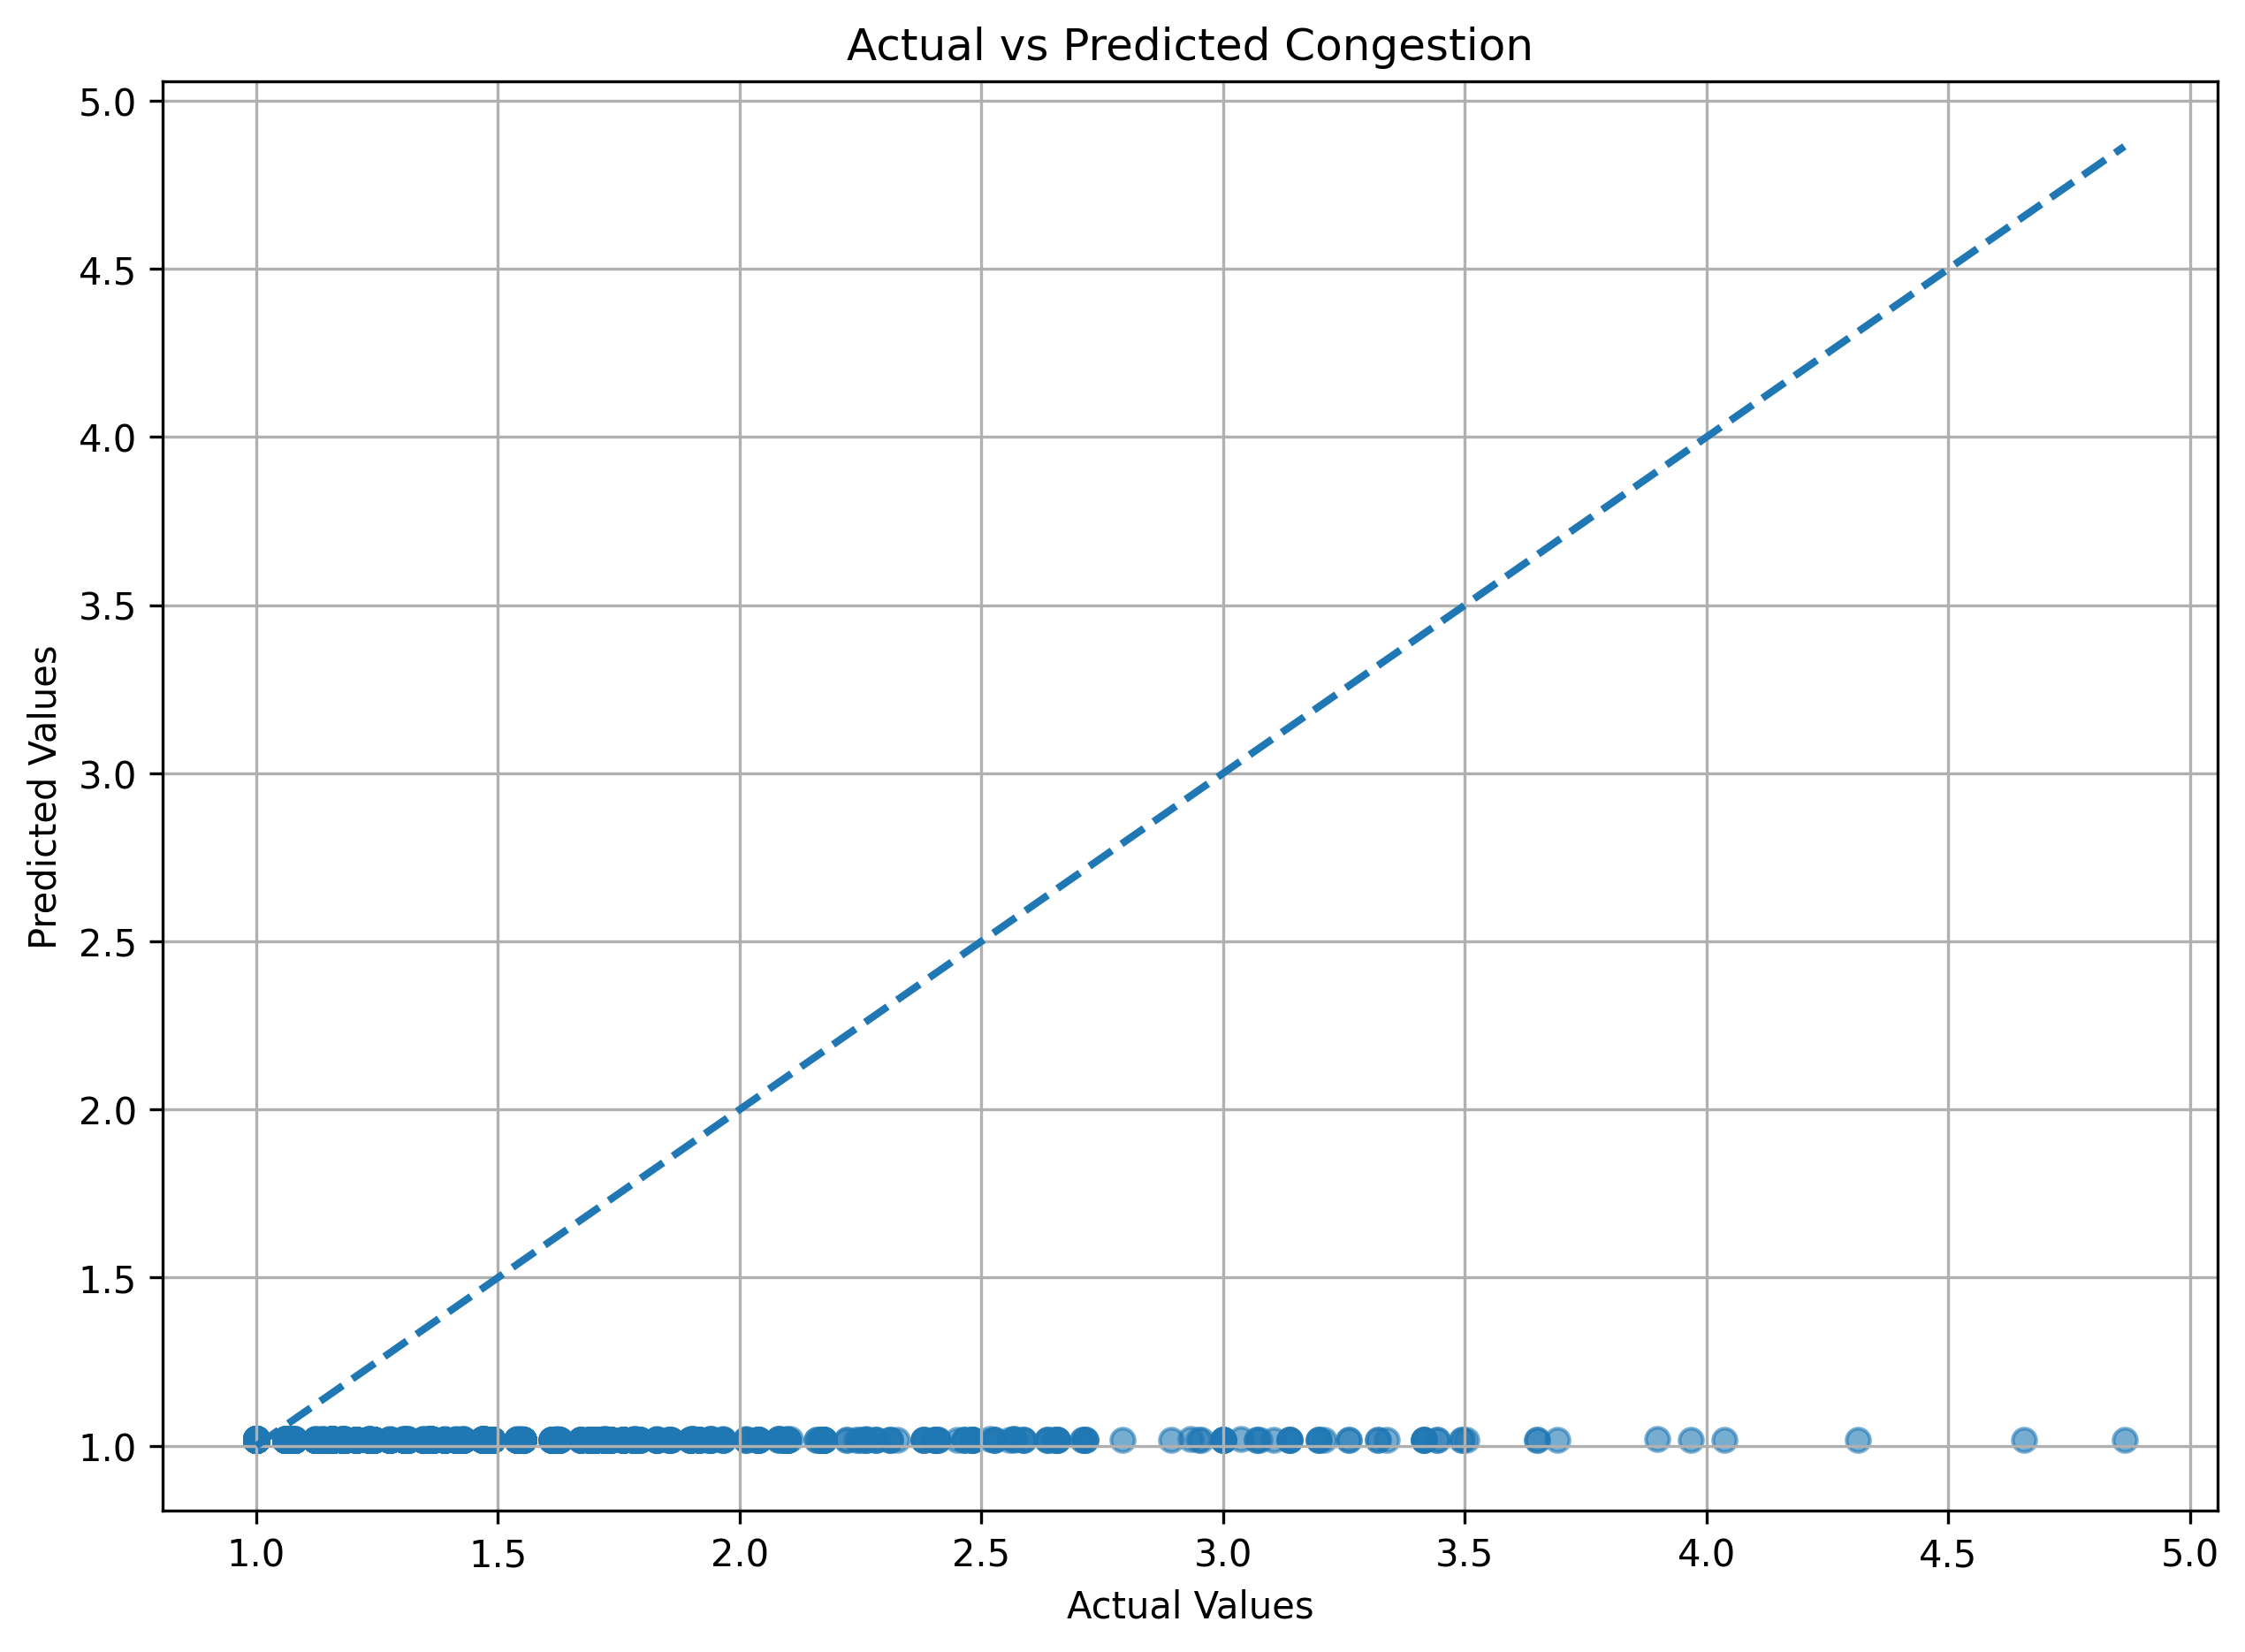
\includegraphics[width=0.72\textwidth]{figures/actual_vs_predicted.png}
\caption[Predicted against actual congestion multipliers]{Predicted against actual congestion multipliers on the test set. The dashed line marks perfect prediction.}
\label{fig:actualpred}
\end{figure}

\begin{table}[htbp]
\centering
\caption{Neural network test-set metrics}
\label{tab:nnmetrics}
\begin{tabular}{lr}
\toprule
Metric & Value \\
\midrule
Mean squared error (MSE) & 0.0895 \\
Root mean squared error (RMSE) & 0.2991 \\
Mean absolute error (MAE) & 0.1130 \\
Coefficient of determination ($R^2$) & $-0.0917$ \\
\bottomrule
\end{tabular}
\end{table}

\section{Summary of Results}

\begin{table}[htbp]
\centering
\caption{Summary of results}
\label{tab:summary}
\small
\begin{tabularx}{\textwidth}{>{\raggedright\arraybackslash}p{3.4cm}X}
\toprule
Question & Finding \\
\midrule
RQ1: Runtime & A* was up to about 30\% slower end to end. \\
RQ1: Route quality & No difference can be attributed to the algorithm: both return minimum-cost routes, re-routing always used Dijkstra's algorithm, and runs used different vehicles. \\
RQ2: Bottlenecks & The busiest single road segment carried 11--13\% of all vehicles at 250 vehicles and above. \\
RQ2: Re-routing & 82--91\% of vehicles changed route in every logged run with 100 or more vehicles; congestion moved to other corridors rather than disappearing. \\
RQ3: Prediction & The network predicted an almost constant 1.02 and scored $R^2 = -0.09$ on the test set. \\
\bottomrule
\end{tabularx}
\end{table}

% ==============================================================================
% CHAPTER 6: DISCUSSION
% ==============================================================================

\chapter{Discussion}
\label{ch:discussion}

\section{Why A* Gave No Benefit}
\label{sec:disc-astar}

A* can only save work when its heuristic is a large fraction of the true remaining cost. Here the heuristic was the straight-line distance between nodes in degrees of longitude and latitude. Oxford spans less than 0.2 degrees in each direction, so the heuristic never exceeded about 0.2, while route costs were several hundred seconds. The heuristic was admissible, because it was far smaller than any real travel time, but it carried almost no information. With $h \approx 0$, A* behaves like one-directional Dijkstra (\cref{eq:astar}). It also pays the cost of a Python function call for every heuristic evaluation.

The baseline it was compared with was stronger than plain Dijkstra. NetworkX's \code{shortest\_path} runs bidirectional Dijkstra for a single source and target, which typically settles far fewer nodes than a one-directional search. A* was therefore slower for two reasons: it searched in one direction instead of two, and it added heuristic overhead without gaining guidance. Runtime also includes work that does not depend on the algorithm (graph loading, Dijkstra re-routing, heat-map rendering and data export), so the difference in search time alone was larger than the end-to-end figures suggest.

An informative and admissible heuristic for travel-time weights is the great-circle distance to the goal divided by the highest speed on any road,
\begin{equation}
h(n) = \frac{d_{\text{gc}}(n, t)}{v_{\max}},
\label{eq:betterh}
\end{equation}
measured in seconds. No route can be shorter than the great-circle distance, and no road can be driven faster than $v_{\max}$, so $h$ never overestimates. Congestion weighting only increases travel times, so the heuristic stays admissible after weights are updated. A fair comparison would also count the nodes each search settles, rather than route length, and time the searches on their own.

\section{Why Re-routing Changed Almost Every Route}
\label{sec:disc-reroute}

The congestion update raises the travel time of every edge that at least one vehicle uses, including edges used only by the vehicle itself. With 100 vehicles, the mean usage $\bar{V}$ was about 2.7 (\cref{tab:explog}). An edge used by a single vehicle therefore has $r_e \approx 0.37$, and by \cref{eq:effective} its travel time rises by about 12\%. Every edge on a vehicle's own route becomes at least that much more expensive, while unused roads keep their baseline cost. Any alternative route within about 12\% of the original's travel time therefore becomes cheaper, and in a dense urban network such alternatives are common. In effect, each vehicle is penalised for its own presence, so most vehicles switch route whether or not their original roads were congested. That explains the 60--91\% re-routing rates in \cref{tab:explog}, including at very light loads.

Re-routing is also simultaneous and happens once. Every vehicle responds to the same snapshot of congestion, so vehicles leaving a busy corridor tend to choose the same alternatives, which then become the new bottlenecks. The heat-maps in \cref{fig:heatmaps} show this. This is the reason traffic-assignment methods iterate, moving only a fraction of traffic at each step until no driver can improve their route, which is Wardrop's user equilibrium \citep{wardrop1952,sheffi1985urban}. Two changes would make the re-routing step more meaningful: exclude each vehicle's own contribution from the usage it sees, and repeat the update with a decreasing step size until routes stop changing.

\section{Topology and Persistent Bottlenecks}

The most robust finding is structural. Whatever the algorithm and after re-routing, the busiest road segment carried a stable 11--13\% of all journeys. With origins and destinations spread uniformly across the city, a large share of journeys must cross a small set of links, such as river crossings and ring-road junctions, that connect otherwise separate parts of the network. Graph theory measures this with betweenness centrality,
\begin{equation}
C_B(v) = \sum_{s \neq v \neq t} \frac{\sigma_{st}(v)}{\sigma_{st}},
\end{equation}
the fraction of shortest paths between all pairs $s, t$ that pass through $v$, where $\sigma_{st}$ is the number of shortest paths from $s$ to $t$ and $\sigma_{st}(v)$ the number of those passing through $v$. Betweenness centrality was not computed in this project. Testing whether the persistent bottlenecks are the edges with the highest betweenness centrality is a natural next step, and it would turn this observation into a measured result \citep{barthelemy2011spatial}.

\section{Why the Neural Network Predicted a Constant}

The network's failure is an optimisation problem, not evidence that the task is hard. The target is an exact function of the inputs. By \cref{eq:multiplier}, the multiplier depends only on edge usage $V_e$, which is the first input feature, and on the run's mean usage $\bar{V}$, which varies between runs. A model given $\bar{V}$ as an extra feature could fit the target almost perfectly, and even a linear regression on the existing features should achieve a clearly positive $R^2$.

The training settings explain the flat prediction. With weights initialised at $0.01 \times \mathcal{N}(0,1)$, the hidden activations are tiny, so the gradients reaching every weight matrix are tiny too. In practice only the output bias $b_3$ receives a usable gradient. After min--max scaling, the mean normalised target is about $(1.11 - 1.0)/3.9 \approx 0.03$. The gradient of the loss with respect to $b_3$ is therefore about $2 \times 0.03 = 0.06$, so with $\eta = 10^{-4}$ the bias moves by about $6 \times 10^{-6}$ per epoch, or about 0.006 over 1,000 epochs. Converted back to the original scale (multiplying by the target range of about 3.9), that is about 0.02. This matches the constant prediction of about 1.02 in \cref{fig:actualpred}. The network had, in effect, learned only its output bias.

Three further factors made the task harder than it needed to be. Most training examples are unused edges with a target of exactly 1.0, so the mean squared error is dominated by them. Full-batch gradient descent takes one step per epoch. And there was no baseline to show that a working model should do far better. The fixes are standard: initialise ReLU layers with variance $2/n_{\text{in}}$ \citep{he2015delving}, raise the learning rate (for example to $10^{-2}$) or use an adaptive optimiser, train with mini-batches until the validation loss stops falling, and compare with a predict-the-mean baseline and a linear regression. Because the target is a known formula, the network can only ever reproduce the existing weighting. A more useful prediction target would be a quantity the simulation does not already compute, such as usage after re-routing predicted from usage before it.

\section{Threats to Validity}
\label{sec:validity}

\begin{itemize}
  \item \textbf{Different vehicles in each run.} No random seed was fixed, so each algorithm was evaluated on a different random set of origins and destinations. Differences between runs are therefore partly sampling variation: two identically configured runs with 100 vehicles differed by 5.6\% in mean travel time (\cref{tab:explog}).
  \item \textbf{Re-routing ignores the algorithm.} Re-routing always uses Dijkstra's algorithm, so every post-re-routing metric (travel cost, edge usage, bottlenecks, re-routed vehicles) is independent of the algorithm that produced the initial routes.
  \item \textbf{Runtime measures the whole pipeline.} Runtime includes graph construction, heat-map rendering and data export, which dilute differences in search time.
  \item \textbf{Search effort was not measured.} The recorded ``nodes explored'' is route length.
  \item \textbf{Repeats and variation.} The number of repeated runs behind each plotted point was not recorded, and no error bars are shown, so small differences between curves should not be interpreted.
  \item \textbf{Separate batches of runs.} The figures come from two sweeps, and the experiment log from an earlier version of the code, so values at matching vehicle counts differ slightly between sources.
\end{itemize}

\section{Limitations of the Model}

\begin{itemize}
  \item \textbf{Static congestion.} Congestion is a count of planned routes, not a dynamic process: there are no queues, traffic signals, departure times or speed--density effects.
  \item \textbf{Uniform random demand.} Origins and destinations are drawn uniformly, whereas real demand concentrates on employment centres, schools and transport hubs, so the location of bottlenecks would differ in practice.
  \item \textbf{No capacity.} Usage is measured relative to the network average, not to each road's capacity, so a busy motorway and a busy residential street are treated alike.
  \item \textbf{One re-routing step.} The simulation does not iterate towards an equilibrium (\cref{sec:disc-reroute}).
\end{itemize}

% ==============================================================================
% CHAPTER 7: CONCLUSION
% ==============================================================================

\chapter{Conclusion}
\label{ch:conclusion}

This project built a congestion-aware routing simulation on Oxford's real road network, using OSMnx and NetworkX, together with a feed-forward neural network written from first principles. The three research questions can now be answered.

\textbf{RQ1.} A* did not reduce routing cost. Its heuristic was measured in degrees while edge costs were in seconds, so it gave almost no guidance, and it was compared against NetworkX's bidirectional Dijkstra. As a result, A* was up to about 30\% slower end to end. Both algorithms return minimum-cost routes, so neither can produce cheaper routes than the other. A properly scaled heuristic (\cref{eq:betterh}) and a direct count of settled nodes are needed for a fair test.

\textbf{RQ2.} Congestion concentrated on a few corridors. From 250 vehicles upwards, the busiest single segment carried 11--13\% of all vehicles, a share that re-routing did not reduce. One round of simultaneous re-routing changed the routes of most vehicles, because each vehicle was penalised for its own presence, and it moved congestion to other corridors rather than removing it. This points to two directions: the network's structure, which betweenness centrality could quantify, and iterative assignment towards an equilibrium.

\textbf{RQ3.} The neural network did not learn the congestion multiplier. It predicted an almost constant 1.02 and scored $R^2 = -0.09$ on held-out data. The cause is identifiable: a learning rate and weight initialisation so small that only the output bias moved during training. The prediction task is itself an exact formula of the inputs, so a correctly trained model should fit it closely; that makes it a useful test of the implementation rather than a prediction problem in its own right.

The project's main value lies in what it reveals about evaluating routing systems: algorithms must be compared on identical journeys, search effort must be measured directly, re-routing needs to iterate, and a learned model needs a baseline before its metrics mean anything.

% ==============================================================================
% CHAPTER 8: FUTURE WORK
% ==============================================================================

\chapter{Future Work}
\label{ch:future}

The following steps are listed in order of priority.

\begin{enumerate}
  \item \textbf{A fair algorithm comparison.} Fix the random seed so that both algorithms route identical vehicles. Use the heuristic of \cref{eq:betterh}. Count settled nodes. Time the searches separately from the rest of the pipeline. Repeat each configuration several times and report means with standard deviations.
  \item \textbf{Use the chosen algorithm for re-routing,} so that post-re-routing metrics reflect it.
  \item \textbf{Iterative re-routing.} Exclude each vehicle's own contribution from the usage it sees, and repeat the congestion update with a decreasing step size until routes stop changing. Measure total travel time (\cref{eq:J}) before and after.
  \item \textbf{Fix the neural network.} Use He initialisation, a larger learning rate or an adaptive optimiser, and mini-batches. Train until the validation loss flattens. Compare against mean and linear-regression baselines. Then choose a target the simulation does not already compute.
  \item \textbf{Evaluate learned weights in the loop.} Compare routing with no re-routing, with the formula weights and with predicted weights.
  \item \textbf{Measure network structure.} Compute edge betweenness centrality and test whether it predicts the persistent bottlenecks.
  \item \textbf{More realistic demand and dynamics.} Add origin--destination demand concentrated on real attractors, road capacities, departure times and, eventually, a traffic simulator.
  \item \textbf{Richer models.} Once the above is in place, graph neural networks \citep{jiang2022gnn} and reinforcement learning \citep{sutton2018reinforcement} are natural extensions, because road networks are graphs and routing is a sequential decision problem.
\end{enumerate}

% ==============================================================================
% REFERENCES
% ==============================================================================

\bibliographystyle{abbrvnat}
\bibliography{refs}

% ==============================================================================
% APPENDIX
% ==============================================================================

\appendix
\chapter{Routing Algorithm Pseudocode}

\begin{algorithm}[H]
\caption{One simulation run with congestion-aware re-routing}
\begin{algorithmic}[1]
\State Build graph $G(V,E)$ with travel times; store $w_e^{\text{base}}$ for every edge
\For{$i = 1$ to $N$}
  \Repeat
    \State Draw random origin $s_i$ and destination $t_i$ from $V$
  \Until{a path from $s_i$ to $t_i$ exists}
  \State $P_i \gets$ fastest path from $s_i$ to $t_i$ (Dijkstra or A*)
\EndFor
\State $V_e \gets$ number of paths $P_i$ that use edge $e$; \quad $\bar{V} \gets$ mean of $V_e$ over used edges
\For{each edge $e$ with $V_e > 0$}
  \State $w_e \gets w_e^{\text{base}}\,(1 + 0.3325\,V_e/\max(\bar{V},1))$ \Comment{multiplier capped at 4.8}
\EndFor
\For{$i = 1$ to $N$}
  \State $P_i \gets$ fastest path from $s_i$ to $t_i$ on updated weights (Dijkstra)
\EndFor
\State Record metrics and heat-maps; export one training example per edge
\end{algorithmic}
\end{algorithm}

\end{document}
